\documentclass{lehramt-informatik}
\InformatikPakete{cpm,mathe,gantt}

\begin{document}

%%%%%%%%%%%%%%%%%%%%%%%%%%%%%%%%%%%%%%%%%%%%%%%%%%%%%%%%%%%%%%%%%%%%%%%%
% Theorie-Teil
%%%%%%%%%%%%%%%%%%%%%%%%%%%%%%%%%%%%%%%%%%%%%%%%%%%%%%%%%%%%%%%%%%%%%%%%

\chapter{CPM-Netzplantechnik}

\begin{quellen}
\item \cite{wiki:netzplantechnik}
\item \cite{wiki:methode-kritischer-pfad}
\end{quellen}

Netzplantechnik, DIN 69900-1

„Netzplantechnik umfasst \memph{alle Verfahren} zur Analyse,
Beschreibung, Planung, Steuerung und Überwachung von \memph{Abläufen}
auf der \memph{Grundlage der Graphentheorie}, wobei Zeit, Kosten,
Einsatzmittel bzw. Ressourcen berücksichtigt werden können. Ein Netzplan
ist die graphische oder tabellarische Darstellung von Abläufen und deren
Abhängigkeiten“.
\footcite[Seite 14]{sosy:fs:3}

CPM: Critical Path Method; Vorgangspfeil-Netzplan

%-----------------------------------------------------------------------
%
%-----------------------------------------------------------------------

\section{Zentrale Begriffe}

Ein \memph{Vorgang} ist eine abgegrenzte Arbeitseinheit mit
\memph{Anfangs- und Endzeit} (vgl. Arbeitspaket im Projektmanagement).
Er besitzt eine \memph{Dauer}.
%
Unter Berücksichtigung der Dauer der einzelnen Vorgänge und unter
Berücksichtigung ihrer Abhängigkeiten wird ermittelt, wann die Vorgänge
stattfinden.
%
In CPM Netzen werden Vorgänge als \memph{Pfeile zwischen Ereignissen}
dargestellt.
\footcite[Seite 15]{sosy:fs:3}

Zweck

Darstellen logischer Zusammenhänge
Zeitplan für alle Vorgänge entwickeln
Kritischer Pfad und Ressourcen-Engpässe identifizieren
Terminüberwachung, laufende Kontrolle
Vier Teilaufgaben:
Kapazitätsplanung
Kostenplanung
Strukturplanung
Zeitplanung/ Zeitfenster
\footcite[Seite 22]{sosy:fs:3}
%-----------------------------------------------------------------------
%
%-----------------------------------------------------------------------

\section{Konstruktion eines Netzes}

Dem Vorgang $A_k$ wird ein Pfeil $e_k$ zugeordnet und mit dessen Dauer
bewertet.
%
$i_k$ und $j_k$ sind Anfangs- und Endereignis.
%
Die Anordnung erfolgt nach der Ende-Start-Beziehung.

\begin{center}
\begin{tikzpicture}
\ereignisN(i){$i_k$}(0,0)
\ereignisN(j){$j_k$}(4,0)
\vorgang(i>j){$e_k$}
\end{tikzpicture}
\end{center}

Regel 1: Folgen die Vorgänge $A_3$ und $A_4$ unmittelbar $A_1$ und $A_2$
so gilt:
\footcite[Seite 24]{sosy:fs:3}

\begin{center}
\begin{tikzpicture}
\ereignisN(1){$i_1$}(0,2)
\ereignisN(2){$i_2$}(0,0)

\ereignisN(m){}(2,1)

\ereignisN(3){$j_3$}(4,2)
\ereignisN(4){$j_4$}(4,0)

\vorgang(1>m){$e_1$}
\vorgang(2>m){$e_2$}
\vorgang(m>3){$e_3$}
\vorgang(m>4){$e_4$}
\end{tikzpicture}
\end{center}

Regel 2: Gibt es zwei Vorgänge (parallele Arbeitspakete) mit demselben
Anfangs- und Endereignis, so wird das Endereignis gesplittet und ein
Scheinvorgang eingeführt:
\footcite[Seite 25]{sosy:fs:3}

\begin{center}
\begin{tikzpicture}
\ereignisN(1){$i_1$}(0,1)
\ereignisN(2){$j_2$}(4,2)
\ereignisN(3){$j_3$}(4,0)

\vorgang(1>2){$e_1$}
\vorgang(1>3){$e_2$}
\scheinvorgang(2>3){$e_0$}
\end{tikzpicture}
\end{center}

Regel 3: Folgt der Vorgange $A_4$ unmittelbar $A_1$ und $A_2$ und folgt
$A_5$ unmittelbar $A_1$ , $A_2$ und $A_3$ so wird ein Scheinvorgang
eingeführt:
\footcite[Seite 26]{sosy:fs:3}

\begin{center}
\begin{tikzpicture}
\ereignisN(1){$i_1$}(0,4)
\ereignisN(2){$i_2$}(0,2)
\ereignisN(3){$i_3$}(0,0)

\ereignisN(4){$j_4$}(4,3)
\ereignisN(5){$j_5$}(4,0)

\ereignisN(m1){}(2,3)
\ereignisN(m2){}(2,0)

\vorgang(1>m1){$e_1$}
\vorgang(2>m1){$e_2$}
\vorgang(3>m2){$e_3$}

\vorgang(m1>4){$e_4$}
\vorgang(m2>5){$e_5$}

\scheinvorgang(m1>m2){$e_0$}
\end{tikzpicture}
\end{center}

Es gibt nur eine Quelle (Projektstart) und eine Senke (Projektende).
Ggf. müssen Scheinvorgänge eingeführt werden, um dies zu erreichen.
%
Kann ein Vorgang $A_2$ bereits begonnen werden, wenn ein Teil des
Vorgangs $A_1$ erledigt ist, so wird $A_1$ gesplittet.\footcite[Seite
27]{sosy:fs:3}

\section{Beispiel\footcite[Seite 16 - 21]{sosy:fs:3}}

\begin{center}
\begin{tikzpicture}
\ereignis{1}(0,2)
\ereignis{2}(1,3.5)
\ereignis{3}(3,2)
\ereignis{4}(2,0.5)
\ereignis{5}(4,3.5)
\ereignis{6}(5,2)
\ereignis{7}(5,0.5)
\ereignis{8}(7.5,2)

\vorgang(1>2){5}
\vorgang(1>3){18}
\vorgang(1>4){7}
\vorgang(4>7){15}
\vorgang(7>8){6}
\vorgang(3>6){8}
\vorgang(3>7){1}
\vorgang(2>5){14}
\vorgang(5>8){11}
\vorgang(6>8){4}
\end{tikzpicture}
\end{center}

\begin{enumerate}

%%
%
%%

\item  Vorwärtsterminierung, $+$, bei Auswahl Maximum
$\text{FZ}_i$ : Frühester Zeitpunkt, zu dem Ereignis $i$ eintreten kann
vgl. FAZ = Frühester AnfangsZeitpunkt für Vorgang
FEZ = Frühester EndeZeitpunkt für Vorgang

%%
%
%%

\item Rückwärtsterminierung, $-$, bei Auswahl Minimum
$\text{SZ}_i$ : Spätester Zeitpunkt, zu dem Ereignis $i$ eintreten kann

vgl. SAZ = Spätester AnfangsZeitpunkt für Vorgang
SEZ = Spätester EndeZeitpunkt für Vorgang

%%
%
%%

\item Puffer

GP: gesamter Pufferzeit ($\text{GP} = \text{SZ} - \text{FZ}$)

%%
%
%%

\item Kritische Pfade
Pfad(e) mit minimaler Pufferzeit, meist $0$

\end{enumerate}

\begin{tabular}{|l|l|l|l|l|l|l|l|l|}
\hline
i             & 1 & 2 & 3  & 4 & 5  & 6  & 7  & 8 \\\hline\hline
$\text{FZ}_i$ & 0 & 5 & 18 & 7 & 19 & 26 & 22 & 30 \\\hline
$\text{SZ}_i$ & 0 & 5 & 18 & 9 & 19 & 26 & 24 & 30 \\\hline
GP            & 0 & 0 & 0  & 2 & 0  & 0  & 2  & 0 \\\hline
\end{tabular}

\bigskip

\begin{tabular}{|l|l|l|}
$\text{FZ}_i$ & Nebenrechnung & \\
1             &  & 0 \\
2             & & 5 \\
3             & & \\
4             & & \\
5             &  & \\
6             & & \\
7             & max(19,22) & \\
8             & max(30,30,38) & 30 \\
\end{tabular}

\bigskip

\begin{tabular}{|l|r|r|}
\hline
$\text{SZ}_i$ & Nebenrechnung & \\
\hline\hline
1             & \f$30 - \t{11}(5-8) - \t{14}(2-5) -\t{5}(1-2) = 0$ & \\
              & \f$30 - \t{4}(6-8) - \t{8}(3-6) - \t{18}(1-3) = 0$ & \\
              & \f$30 - \t{6}(7-8) - \t{15}(4-7) - \t{7}(1-4) = 2$ & \\
              & \f$\min(0,0,2)$ & 0 \\\hline

2             & \f$30 - \t{11}(5-8) - \t{14}(2-5) = 5$ & 5 \\\hline
3             & \f$30 - \t{4}(6-8) - \t{8}(3-6) = 18$  & \\
              & \f$30 - \t{6}(7-8) - \t{1}(3-7) = 23$  & \\
              & \f$\min(18,23)$                        & 18 \\\hline

4             & \f$30 - \t{6}(7-8) - \t{15}(4-7)$      & 9 \\\hline
5             & \f$30 - \t{11}(5-8)$                   & 19 \\\hline
6             & \f$30 - \t{4}(6-8)$                    & 26 \\\hline
7             & \f$30 - \t{6}(7-8)$                    & 24 \\\hline
8             & \f{}siehe $\text{FZ}_8$                & 30 \\\hline
\end{tabular}

%%%%%%%%%%%%%%%%%%%%%%%%%%%%%%%%%%%%%%%%%%%%%%%%%%%%%%%%%%%%%%%%%%%%%%%%
% Aufgaben
%%%%%%%%%%%%%%%%%%%%%%%%%%%%%%%%%%%%%%%%%%%%%%%%%%%%%%%%%%%%%%%%%%%%%%%%

\chapter{Aufgaben}

\section{Aufgabe 1: CPM-Netzplantechnik\footcite[Seite 1]{sosy:ab:5}}

Gegeben ist das nachfolgende CPM-Netz. Gestrichelte Linien zwischen
Ereignissen stellen Scheinvorgänge mit einer Dauer von $0$ dar.

\begin{center}
\begin{tikzpicture}
\ereignis{1}(-1,2)
\ereignis{2}(1,4)
\ereignis{3}(1,0)
\ereignis{4}(3,2)
\ereignis{5}(5,4)
\ereignis{6}(5,0)
\ereignis{7}(7,2)
\ereignis{8}(9,4)
\ereignis{9}(9,0)
\ereignis{10}(11,2)

\vorgang(1>2){2}
\vorgang(1>3){3}
\vorgang(2>5){4}
\vorgang(3>4){4}
\vorgang(3>6){3}
\vorgang(4>5){1}
\vorgang(5>7){3}
\vorgang(5>8){2}
\vorgang(6>7){3}
\vorgang(7>10){1}
\vorgang(7>9){2}
\vorgang(9>10){3}

\scheinvorgang(1>4){}
\scheinvorgang(4>6){}
\scheinvorgang(6>9){}
\scheinvorgang(8>10){}
\end{tikzpicture}
\end{center}

\begin{enumerate}

%%
% (a)
%%

\item Begründen Sie, welche Scheinvorgänge aus dem Netzplan ohne
Informationsverlust gestrichen werden könnten.

\begin{antwort}
Die Scheinvorgänge zwischen den Ereignissen $1$ und $4$ bzw. zwischen $6$ und
$9$ können jeweils gestrichen werden, da Ereignis $4$ schon auf $1$ wartet
(über $3$) und $9$ wartet auf $6$ (über $7$).
\end{antwort}

%%
% (b)
%%

\item Berechnen Sie für jedes Ereignis den \emph{frühesten Termin}, den
\emph{spätesten Termin} sowie die \emph{Gesamtpufferzeiten}.

\begin{antwort}
\begin{tabular}{|l|r|r|}
\hline
$\text{FZ}_i$ & Nebenrechnung & \\\hline\hline
1 &                                                       & $0$ \\\hline
2 &                                                       & $2$ \\\hline
3 &                                                       & $3$ \\\hline
4 &                                                       & $7$ \\\hline
5 & \f$\max(\v{3}(3) + 3,\v{7}(4) + 1)$                   & $8$ \\\hline
6 & \f$\max(\v{3}(3) + 3,\v{7}(4) + 0)$                   & $7$ \\\hline
7 & \f$\max(\v{8}(5) + 3,\v{7}(6) + 3)$                   & $11$ \\\hline
8 & \f$\v{8}(5) + 2$                                      & $10$ \\\hline
9 & \f$\max(\v{7}(6) + 0,\v{11}(7) + 2)$                  & $13$ \\\hline
10 & \f$\max(\v{10}(7) + 1, \v{8}(8) + 0, \v{13}(9) + 3)$ & $16$ \\\hline
\end{tabular}

\begin{tabular}{|l|r|r|}
\hline
$\text{FZ}_i$ & Nebenrechnung & \\\hline\hline
1 &                                         & $0$ \\\hline
2 & \f$\max(\v{8}(5) - 4$                   & $4$ \\\hline
3 & \f$\max(\v{8}(6) - 3,\v{7}(4) - 4)$     & $3$ \\\hline
4 & \f$\max(\v{8}(5) - 1,\v{8}(6) - 0)$     & $7$ \\\hline
5 & \f$\max(\v{16}(8) - 2,\v{11}(7) - 3)$   & $8$ \\\hline
6 & \f$\max(\v{11}(7) - 3,\v{13}(9) - 0)$   & $8$ \\\hline
7 & \f$\min(\v{16}(10) - 1, \v{13}(9) - 2)$ & $11$ \\\hline
8 & \f$\v{16}(10) - 0$                      & $16$ \\\hline
9 & \f$\v{16}(10) - 3$                      & $13$ \\\hline
10 & \f{}siehe $\text{FZ}_10$               & $16$ \\\hline
\end{tabular}

\begin{tabular}{|l|l|l|l|l|l|l|l|l|l|l|}
\hline
i             & 1 & 2  & 3   & 4  & 5  & 6  & 7  & 8  & 9  & 10 \\\hline\hline
$\text{FZ}_i$ & 0 & 2  & 3   & 7  & 8  & 7  & 11 & 10 & 13 & 16 \\\hline
$\text{SZ}_i$ & 0 & 4  & 3   & 7  & 8  & 8  & 11 & 16 & 13 & 16 \\\hline
GP            & 0 & 2  & 0   & 0  & 0  & 1  & 0  & 6  & 0  & 0 \\\hline
\end{tabular}
\end{antwort}

%%
% (c)
%%

\item Bestimmen Sie den kritischen Pfad.

\begin{antwort}
$1 \rightarrow 3 \rightarrow 4 \rightarrow 5 \rightarrow 7 \rightarrow 9 \rightarrow 10$

\begin{center}
\begin{tikzpicture}[scale=0.8,transform shape]
\ereignis{1}(-1,2)
\ereignis{2}(1,4)
\ereignis{3}(1,0)
\ereignis{4}(3,2)
\ereignis{5}(5,4)
\ereignis{6}(5,0)
\ereignis{7}(7,2)
\ereignis{8}(9,4)
\ereignis{9}(9,0)
\ereignis{10}(11,2)

\vorgang(1>2){2}
\VORGANG(1>3){3}
\vorgang(2>5){4}
\VORGANG(3>4){4}
\vorgang(3>6){3}
\VORGANG(4>5){1}
\VORGANG(5>7){3}
\vorgang(5>8){2}
\vorgang(6>7){3}
\vorgang(7>10){1}
\VORGANG(7>9){2}
\VORGANG(9>10){3}

\scheinvorgang(1>4){}
\scheinvorgang(4>6){}
\scheinvorgang(6>9){}
\scheinvorgang(8>10){}
\end{tikzpicture}
\end{center}
\end{antwort}
\end{enumerate}

%-----------------------------------------------------------------------
%
%-----------------------------------------------------------------------

\section{Aufgabe 4 (Check-Up)\footcite[Seite 2]{sosy:ab:5}}
% korrigiert 8.9.2020

\begin{enumerate}

%%
% (a)
%%

\item Gegeben ist folgender (unvollständiger) CPM-Netzplan, sowie die
frühesten und spätesten Termine und die Pufferzeiten aller Ereignisse:

\begin{minipage}{4cm}
\begin{tikzpicture}
\ereignis{1}(0,1)
\ereignis{2}(1,1)
\ereignis{3}(2,2)
\ereignis{4}(2,0)
\ereignis{5}(3,1)

\vorgang(1>2){}
\vorgang(2>3){}
\vorgang(2>4){}
\vorgang(4>5){}
\vorgang(3>5){}

\scheinvorgang(3>4){}
\end{tikzpicture}
\end{minipage}
%
\begin{minipage}{5cm}
\begin{tabular}{|l|l|l|l|l|l|}
\hline
Ereignis         & 1 & 2 & 3 & 4 & 5 \\\hline\hline
frühester Termin & 0 & 1 & 2 & 4 & 8 \\\hline
spätester Termin & 0 & 1 & 2 & 5 & 8 \\\hline
Puffer           & 0 & 0 & 0 & 1 & 0 \\\hline
\end{tabular}
\end{minipage}

Vervollständigen Sie den CPM-Netzplan, indem Sie mit Hilfe obiger
Tabelle die Zeiten der Vorgänge berechnen.

\begin{antwort}
\begin{tikzpicture}
\ereignis{1}(0,1)
\ereignis{2}(1,1)
\ereignis{3}(2,2)
\ereignis{4}(2,0)
\ereignis{5}(3,1)

\vorgang(1>2){1}
\vorgang(2>3){1}
\vorgang(2>4){3}
\vorgang(4>5){3}
\vorgang(3>5){6}

\scheinvorgang(3>4){}
\end{tikzpicture}

%%
%
%%

\ueberschrift{Frühester Termin/Zeitpunkt}

\begin{tabular}{|l|r|r|}
\hline
$\text{FZ}_i$ & Nebenrechnung & \\
\hline\hline
1             &                               & 0 \\\hline
2             & \f$0 + \t{1}(1-2) = 1$          & 1 \\\hline
3             & \f$\t{1}(1-2) + \t{1}(2-3) = 2$ & 2 \\\hline
4             & \f$\t{1}(1-2) + \t{3}(2-4) = 4$ &  \\
              & \f$\t{1}(1-2) + \t{1}(2-3) + \t{0}(3-4) = 2$ & \\
              & \f$\max(4,2)$                   & 4 \\\hline

5             & \f$\f\t{1}(1-2) + \t{1}(2-3) + \t{6}(3-5) = 8$ & \\
              & \f$\t{1}(1-2) + \t{3}(2-4) + \t{3}(4-5) = 7$ & \\
              & \f$\max(8,7)$                   & 8 \\\hline

\end{tabular}

%%
%
%%

\ueberschrift{Spätester Termin/Zeitpunkt}

\begin{tabular}{|l|r|r|}
\hline
$\text{SZ}_i$ & Nebenrechnung & \\
\hline\hline
1             & \f$8 - \t{6}(3-5) - \t{1}(2-3) - \t{1}(1-2) = 0$ & \\
              & \f$8 - \t{3}(4-5) - \t{3}(2-4) - \t{1}(1-2) = 1$ & \\
              & \f$\min(0,1)$ & 0 \\\hline

2             & \f$8 - \t{6}(3-5) - \t{1}(2-3) = 1$ & \\
              & \f$8 - \t{3}(4-5) - \t{3}(2-4) = 2$ & \\
              & \f$\min(1,2)$ & 1 \\\hline

3             & \f$8 - \t{6}(3-5) = 2$ & 2  \\\hline

4             & \f$8 - \t{3}(4-5) = 5$      & 3 \\\hline
5             & \f{}siehe $\text{FZ}_5$  & 8 \\\hline
\end{tabular}
\end{antwort}

%%
% (b)
%%

\item Bestimmen Sie zum nachfolgenden CPM-Netzplan für jedes Ereignis
den \emph{frühesten Termin}, den \emph{spätesten Termin} sowie die
\emph{Gesamtpufferzeit}. Geben Sie außerdem den \emph{kritischen Pfad}
an.

\begin{center}
\begin{tikzpicture}
\ereignis{1}(0,2)
\ereignis{2}(2,4)
\ereignis{3}(2,0)
\ereignis{4}(4,2)
\ereignis{5}(6,4)
\ereignis{6}(6,0)
\ereignis{7}(8,2)

\vorgang(1>2){4}
\vorgang(1>3){8}
\vorgang(2>3){5}
\vorgang(2>4){7}
\vorgang(2>5){8}
\vorgang(3>4){1}
\vorgang(3>6){6}
\vorgang(4>5){2}
\vorgang(4>6){5}
\vorgang(5>6){6}
\vorgang(5>7){7}
\vorgang(6>7){2}
\end{tikzpicture}
\end{center}

\begin{antwort}
\begin{tabular}{|l|l|l|l|l|l|l|l|}
\hline
i             & 1 & 2 & 3  & 4 & 5  & 6  & 7  \\\hline\hline
$\text{FZ}_i$ & 0 & 4 & 9  & 11 & 13 & 19 & 21  \\\hline
$\text{SZ}_i$ & 0 & 4 & 10 & 11 & 13 & 19 & 21  \\\hline
GP            & 0 & 0 & 1  & 0  & 0  & 0  & 0  \\\hline
\end{tabular}

%%
%
%%

\ueberschrift{Frühester Termin/Zeitpunkt}

\begin{tabular}{|l|r|r|}
\hline
$\text{FZ}_i$ & Nebenrechnung & \\
\hline\hline
1 &                                                                      & 0 \\\hline
2 &                                                                      & 4 \\\hline
3 & \f$\max(8, \v{4}(2) + 5) = \max(8, 9)$                                      & 9 \\\hline
4 & \f$\max(\v{9}(3) + 1, \v{4}(2) + 7) = \max(10, 11)$                    & 11 \\\hline
5 & \f$\max(\v{4}(2) + 8, \v{11}(4) + 2) = \max(12, 13)$                   & 13 \\\hline
6 & \f$\max(\v{13}(5) + 6, \v{11}(4) + 5, \v{9}(3) + 6) = \max(19, 16, 15)$ & 19 \\\hline
7 & \f$\max(\v{13}(5) + 7, \v{19}(6) + 2) = \max(20, 21)$                  & 21 \\\hline
\end{tabular}

%%
%
%%

\ueberschrift{Spätester Termin/Zeitpunkt}

\begin{tabular}{|l|r|r|}
\hline
$\text{SZ}_i$ & Nebenrechnung & \\
\hline\hline
1 & \f$\min(\v{4}(2) - 4, \v{10}(3) - 8) = \min(0, 2)$                    & 0 \\\hline
2 & \f$\min(\v{13}(5) - 8, \v{11}(4) - 7, \v{10}(3) - 5) = \min(5, 4, 5)$ & 4\\\hline
3 & \f$\min(\v{11}(4) - 1, \v{19}(6) - 6) = \min(10, 13)$                 & 10 \\\hline
4 & \f$\min(\v{13}(5) - 2, \v{19}(6) - 5) = \min(11, 14)$                 & 11 \\\hline
5 & \f$\min(\v{21}(7) - 7, \v{19}(6) - 6) = \min(14, 13)$                 & 13 \\\hline
6 & \f$\v{21}(7) - 2$                                                     & 19 \\\hline
7 & \f{}siehe $\text{FZ}_7$                                               & 21 \\\hline
\end{tabular}

%%
%
%%

\ueberschrift{Kritischer Pfad}

$1 \rightarrow 2 \rightarrow 4 \rightarrow 5 \rightarrow 6 \rightarrow 7$

$\t{4}(1-2) + \t{7}(2-4) + \t{2}(4-5) + \t{6}(5-6) + \t{2}(6-7) = 21$

\begin{center}
\begin{tikzpicture}[scale=0.8,transform shape]
\ereignis{1}(0,2)
\ereignis{2}(2,4)
\ereignis{3}(2,0)
\ereignis{4}(4,2)
\ereignis{5}(6,4)
\ereignis{6}(6,0)
\ereignis{7}(8,2)

\VORGANG(1>2){4}
\vorgang(1>3){8}
\vorgang(2>3){5}
\VORGANG(2>4){7}
\vorgang(2>5){8}
\vorgang(3>4){1}
\vorgang(3>6){6}
\VORGANG(4>5){2}
\vorgang(4>6){5}
\VORGANG(5>6){6}
\vorgang(5>7){7}
\VORGANG(6>7){2}
\end{tikzpicture}
\end{center}
\end{antwort}

%%
% (c)
%%

\item Konvertieren Sie das nachfolgende Gantt-Diagramm in ein
CPM-Netzwerk. Als Hilfestellung ist die Anordnung der Ereignisse bereits
vorgegeben.

\begin{center}
\begin{ganttchart}[x unit=1cm, y unit chart=0.8cm]{0}{9}
\gantttitlelist{0,...,9}{1} \\
\ganttbar[name=A]{A}{0}{2} \\
\ganttbar[name=B]{B}{1}{4} \\
\ganttbar[name=C]{C}{3}{4} \\
\ganttbar[name=D]{D}{6}{8}

\node at (A) {3};
\node at (B) {4};
\node at (C) {2};
\node at (D) {3};

\ganttlink[link type=s-s]{A}{B}
\ganttlink[link type=f-s]{A}{C}
\ganttlink[link type=f-f]{B}{D}
\ganttlink[link type=s-f]{B}{C}
\ganttlink[link type=s-s]{C}{D}
\end{ganttchart}
\end{center}

\begin{antwort}
\begin{center}
\begin{tikzpicture}[scale=0.8,transform shape]
\ereignis{SP}(-1.5,2)

\ereignis{A1}(0,2)
\ereignis{A2}(1.5,4)
\ereignis{B1}(1.5,0)
\ereignis{B2}(6,0)
\ereignis{C1}(3,4)
\ereignis{C2}(5.5,1.5)
\ereignis{D1}(6,4)
\ereignis{D2}(7.5,2.5)

\ereignis{EP}(9,2)

\vorgang(A1>A2){3}
\vorgang(A1>B1){1}
\vorgang(B1>B2){4}
\vorgang(B1>C2){4}
\vorgang(C1>C2){2}
\vorgang(C1>D1){3}
\vorgang(D1>D2){3}

\scheinvorgang(A2>C1){}
\scheinvorgang(B2>D2){}
\scheinvorgang(D2>EP){}
\scheinvorgang(C2>EP){}
\scheinvorgang(SP>A1){}
\end{tikzpicture}
\end{center}
\end{antwort}
\end{enumerate}

%-----------------------------------------------------------------------
%
%-----------------------------------------------------------------------

\section{2 Projektmanagement}

Abbildung 2 stellt ein CPM-Netzwerk dar. Die Ereignisse sind fortlaufend
nummeriert (Nummer im Inneren der Kreise) und tragen keine Namen.
Gestrichelte Linien stellen Pseudo-Aktivitäten mit einer Dauer von 0
dar.\footcite{examen:66116:2012:09}

\begin{center}
\begin{tikzpicture}
\ereignis{1}(0,2)
\ereignis{2}(1,4)
\ereignis{3}(1,0)
\ereignis{4}(3,4)
\ereignis{5}(3,2)
\ereignis{6}(3,0)
\ereignis{7}(5,4)
\ereignis{8}(5,2)
\ereignis{9}(5,0)
\ereignis{10}(7,2)

\vorgang(1>2){10}
\vorgang(1>3){22}
\vorgang(1>5){6}
\vorgang(1>6){5}
\vorgang(2>4){8}
\vorgang(2>5){5}
\vorgang(3>6){8}
\vorgang(4>5){1}
\vorgang(4>7){12}
\vorgang(6>9){11}
\vorgang(7>10){6}
\vorgang(7>8){3}
\vorgang(8>10){7}
\vorgang(9>10){9}

\scheinvorgang(5>6){}
\scheinvorgang(5>8){}
\end{tikzpicture}
\end{center}

\begin{enumerate}

%%
% 1.
%%

\item Berechnen Sie die früheste Zeit für jedes Ereignis, wobei
angenommen wird, dass das Projekt zum Zeitpunkt 0 startet! (5 Punkte)

\begin{antwort}
\begin{tabular}{|l|r|r|}
\hline
$\text{FZ}_i$ & Nebenrechnung & \\\hline\hline
1 &                                                                           & $0$ \\\hline
2 &                                                                           & $10$ \\\hline
3 &                                                                           & $22$ \\\hline
4 & \f$\t{10}(1-2) + \t{8}(2-4) $                                             & $18$ \\\hline
5 & \f$\max(\v{10}(2) + 5,\v{6}(1),\v{18}(4) + 1) = \max(15,6,19)$            & $19$ \\\hline
6 & \f$\max(\v{5}(1),\v{22}(3) + 8, \v{19}(5) + 0) = \max(5, 30, 19)$         & $30$ \\\hline
7 & \f$\v{18}(4) + 12$                                                        & $30$ \\\hline
8 & \f$\max(\v{30}(7) + 3, \v{19}(5) + 0) = \max(33,19)$                      & $33$ \\\hline
9 & \f$\v{30}(6) + 11$                                                        & $41$ \\\hline
10 & \f$\max(\v{30}(7) + 6, \v{33}(8) + 7, \v{41}(9) + 9) = \max(36, 40, 50)$ & $50$ \\\hline
\end{tabular}
\end{antwort}

%%
% 2.
%%

\item Setzen Sie anschließend beim letzten Ereignis die späteste Zeit
gleich der frühesten Zeit und berechnen Sie die spätesten Zeiten! (5
Punkte)

\begin{antwort}
\begin{tabular}{|l|r|r|}
\hline
$\text{SZ}_i$ & Nebenrechnung & \\\hline\hline
1 & & $0$ \\\hline
2 & \f$\min(\v{28}(v) - 8, \v{30}(5) - 5)$               & $20$ \\\hline
3 & \f$\v{30}(6) - 8$                                    & $22$ \\\hline
4 & \f$\min(\v{30}(6) - 0, \v{40}(7) - 12)$              & $28$ \\\hline
5 & \f$\min(\v{30}(5) - 1, \v{43}(8) - 0)$               & $30$ \\\hline
6 & \f$\v{41}(9) - 11$                                   & $30$ \\\hline
7 & \f$\min(\v{50}(10) - 6, \v{43}(8) - 3) \min(44, 40)$ & $40$ \\\hline
8 & \f$\v{50}(10) - 7$                                   & $43$ \\\hline
9 & \f$\v{50}(10) - 9$                                   & $41$ \\\hline
10 & \f{}siehe $\text{FZ}_10$                            & $50$ \\\hline
\end{tabular}
\end{antwort}

%%
% 3.
%%

\item Berechnen Sie nun für jedes Ereignis die Pufferzeiten! (5 Punkte)

\begin{antwort}
\begin{tabular}{|l|l|l|l|l|l|l|l|l|l|l|}
\hline
i             & 1 & 2  & 3   & 4  & 5  & 6  & 7  & 8  & 9  & 10 \\\hline\hline
$\text{FZ}_i$ & 0 & 10 & 22  & 18 & 19 & 30 & 30 & 33 & 41 & 50 \\\hline
$\text{SZ}_i$ & 0 & 20 & 22  & 28 & 30 & 30 & 40 & 43 & 41 & 50 \\\hline
GP            & 0 & 10 & 0   & 10 & 11 & 0  & 10 & 10 & 0  & 0 \\\hline
\end{tabular}
\end{antwort}

%%
% 4.
%%

\item Bestimmen Sie den kritischen Pfad! (2 Punkte)

\begin{antwort}
$1 \rightarrow 3 \rightarrow 6 \rightarrow 9 \rightarrow 10$

\begin{center}
\begin{tikzpicture}[scale=0.8,transform shape]
\ereignis{1}(0,2)
\ereignis{2}(1,4)
\ereignis{3}(1,0)
\ereignis{4}(3,4)
\ereignis{5}(3,2)
\ereignis{6}(3,0)
\ereignis{7}(5,4)
\ereignis{8}(5,2)
\ereignis{9}(5,0)
\ereignis{10}(7,2)

\vorgang(1>2){10}
\VORGANG(1>3){22}
\vorgang(1>5){6}
\vorgang(1>6){5}
\VORGANG(3>6){8}
\vorgang(2>5){5}
\vorgang(2>4){8}
\vorgang(4>7){12}
\vorgang(7>8){3}
\vorgang(7>10){6}
\VORGANG(9>10){9}
\VORGANG(6>9){11}
\vorgang(8>10){7}
\vorgang(4>5){1}

\scheinvorgang(5>6){}
\scheinvorgang(5>8){}
\end{tikzpicture}
\end{center}
\end{antwort}

%%
% 5.
%%

\item Konvertieren Sie das Gantt-Diagramm aus Abbildung 3 in ein
CPM-Netzwerk! (10 Punkte)

\begin{center}
\begin{ganttchart}[x unit=0.75cm, y unit chart=0.8cm]{0}{11}
\gantttitlelist{0,...,11}{1} \\
\ganttbar[name=1]{1}{0}{1} \\
\ganttbar[name=2]{2}{2}{4} \\
\ganttbar[name=3]{3}{3}{3} \\
\ganttbar[name=4]{4}{6}{7} \\
\ganttbar[name=5]{5}{7}{11}

\node at (1) {2};
\node at (2) {3};
\node at (3) {1};
\node at (4) {2};
\node at (5) {5};

\ganttlink[link type=f-f]{3}{2}
\ganttlink[link type=f-s]{1}{2}
\ganttlink[link type=f-s]{1}{3}
\ganttlink[link type=f-s]{2}{4}
\ganttlink[link type=s-s]{4}{5}
\end{ganttchart}
\end{center}

\begin{antwort}
\begin{center}
\begin{tikzpicture}
\ereignis{SP}(-6,0)
\ereignis{S1}(-5,1.5)
\ereignis{E1}(-4.5,0)
\ereignis{S2}(-3,1.5)
\ereignis{E2}(-1.5,1.5)
\ereignis{S3}(-3,0)
\ereignis{E3}(-1.75,0)
\ereignis{S4}(0,1.5)
\ereignis{E4}(1.5,1.5)
\ereignis{S5}(0.5,0)
\ereignis{E5}(2,0)
\ereignis{EP}(3.5,0)

\vorgang(S1>E1){2}
\vorgang(S2>E2){3}
\vorgang(S3>E3){1}
\vorgang(S4>E4){2}
\vorgang(S5>E5){5}

\scheinvorgang(SP>S1){}
\scheinvorgang(E5>EP){}
\scheinvorgang(E1>S2){}
\vorgang(E1>S3){1}
\vorgang(E3>E2){1}
\vorgang(E2>S4){1}
\vorgang(S4>S5){1}
\scheinvorgang(E4>EP){}
\end{tikzpicture}
\end{center}
\end{antwort}
\end{enumerate}

%-----------------------------------------------------------------------
%
%-----------------------------------------------------------------------

\section{3. Projektmanagement\footcite{sosy:pu:4}}

Betrachten Sie folgendes CPM-Netzwerk:\footcite{examen:46116:2015:09}

\begin{center}
\begin{tikzpicture}
\ereignis{A}(0,4)
\ereignis{B}(2,4)
\ereignis{C}(0,2)
\ereignis{D}(2,2)
\ereignis{E}(4,3)
\ereignis{F}(6,3)
\ereignis{G}(8,3)
\ereignis{H}(8,1)
\ereignis{I}(10,1)
\ereignis{J}(10,3)

\vorgang(A>B){4}
\vorgang(C>D){1}
\vorgang(E>F){5}
\vorgang(G>J){8}
\vorgang(H>I){9}
\vorgang(J>I){2}

\scheinvorgang(A>C){}
\scheinvorgang(B>E){}
\scheinvorgang(D>E){}
\scheinvorgang(F>G){}
\scheinvorgang(G>H){}
\end{tikzpicture}
\end{center}
\begin{enumerate}

%%
% a)
%%

\item Berechnen Sie die früheste Zeit für jedes Ereignis, wobei
angenommen wird, dass das Projekt zum Zeitpunkt 0 startet.

%%
% b)
%%

\item Setzen Sie anschließend beim letzten Ereignis die späteste Zeit
gleich der frühesten Zeit und berechnen Sie die spätesten Zeiten.

%%
% c)
%%

\item Berechnen Sie nun für jedes Ereignis die Pufferzeiten.

%%
% d)
%%

\item Bestimmen Sie den kritischen Pfad.

%%
% e)
%%

\item Was ist ein Gantt-Diagramm? Worin unterscheidet es sich vom
CPM-Netzwerk?

\end{enumerate}

\literatur

\end{document}
